\documentclass[a4paper,12pt]{article} 
\usepackage{geometry}
\usepackage{wrapfig}
\geometry{
	a4paper,
	total={170mm,257mm},
	left=10mm,
	right=10mm,
	top=20mm,
}
\usepackage{titlesec}
\titlelabel{\thetitle.\quad} %точка в section

%%% Работа с русским языком
\usepackage{cmap}                           % поиск в PDF
\usepackage{mathtext} 			 	       % русские буквы в формулах
\usepackage[T2A]{fontenc}               % кодировка
\usepackage[utf8]{inputenc}              % кодировка исходного текста
\usepackage[english,russian]{babel}  % локализация и переносы

%Математика
\usepackage{amsmath,amsfonts,amssymb,amsthm,mathtools} % AMS
\usepackage{icomma} % "Умная" запятая

%% Шрифты
\usepackage{euscript}	 % Шрифт Евклид
\usepackage{mathrsfs} % Красивый матшрифт

\usepackage{gensymb}
\usepackage{graphicx}
\usepackage{setspace}
\usepackage{tabularx}
\usepackage{longtable}
\usepackage{icomma}
\usepackage{euscript}
\usepackage{float}
\usepackage{cutwin}
\usepackage{adjustbox}
\usepackage{dashbox}
\usepackage[normalem]{ulem}	
\usepackage[babel=true]{microtype}
\RequirePackage[T1]{fontenc}
\usepackage{amsmath,amsfonts,amssymb,amsthm,mathrsfs,mathtools} 
\usepackage{xcolor}         
\usepackage{enumitem}     
\usepackage{xpatch}       
\usepackage{cancel}                  
\usepackage{upgreek}                 
\usepackage{lipsum}                  
\usepackage[version=4]{mhchem}       
\usepackage{multirow}                
\usepackage{stackengine}             
\usepackage{tikz}         
\usepackage{hyperref}
\hypersetup{colorlinks=true,urlcolor=blue}       
\usetikzlibrary{positioning}         
\usepackage{titletoc}                 
\usepackage{chngcntr}              
\usepackage{fancyhdr}                
\usepackage{makecell}                
\usepackage{indentfirst}             
\usepackage{tocloft}                 
\usepackage{soul}                   
\usepackage[stable]{footmisc}       
\usepackage{subfig}  
\usepackage{comment}                  


\mathtoolsset{showonlyrefs=true}


\theoremstyle{definition}
\newtheorem*{definition}{Определение}
\newtheorem{statement}{Предложение}[section]
\newtheorem{lemma}{Лемма}[section]
\newtheorem{theorem}{Теорема}[section]
\newtheorem*{theoremn}{Теорема}
\newtheorem*{corollary}{Следствие}
\newtheorem*{example}{Пример}
\newtheorem*{note}{Замечание}
\newtheorem*{problem}{Задача}


\counterwithout{footnote}{section}\DeclareRobustCommand{\divby}{%
	\mathrel{\text{\vbox{\baselineskip.65ex\lineskiplimit0pt\hbox{.}\hbox{.}\hbox{.}}}}%
}

\newcommand{\dotpr}[2]{\bra{#1}\ket{#2}}
\let\AA\relax
\let\emptyset\varnothing
\DeclareMathOperator*{\esssup}{ess sup}
\DeclareMathOperator*{\ord}{ord}
\DeclareMathOperator*{\supp}{supp}
\DeclareMathOperator*{\pr}{pr}
\DeclareMathOperator*{\Ker}{Ker}
\DeclareMathOperator*{\Vol}{Vol}
\DeclareMathOperator*{\rg}{rk}
\DeclareMathOperator*{\Ima}{Im}
\DeclareMathOperator*{\Alt}{Alt}
\DeclareMathOperator*{\Sym}{Sym}
\newcommand{\eqdef}{\stackrel{\text{\tiny{def}}}{=}}
\newcommand{\pp}{\partial}
\newcommand{\AA}{\mathcal{A}}
\newcommand{\BB}{\mathcal{B}}
\newcommand{\MM}{\mathbb{M}}
\newcommand{\NN}{\mathbb{N}}
\newcommand{\ZZ}{\mathbb{Z}}
\newcommand{\QQ}{\mathbb{Q}}
\newcommand{\RR}{\mathbb{R}}
\newcommand{\CC}{\mathbb{C}}
\newcommand{\FFF}{\mathbb{F}}
\newcommand{\DD}{\mathcal{D}}
\newcommand{\FF}{\mathcal{F}}
\newcommand{\sS}{\mathcal{S}}
\newcommand*\circled[1]{\tikz[baseline=(char.base)]{
		\node[shape=circle,draw,inner sep=2pt] (char) {#1};}}

\author{Шерхалов Денис Б02-204 \\
        Фаттахов Марат Б02-204}
\title{Лабораторная работа 3.3.5 \\
	\textbf{Эффект Холла в металлах}}
\date{\today}


\begin{document}
	
{\Large \maketitle}

\paragraph*{Цель работы:} измерение подвижности и концентрации носителей заряда в металлах.
\paragraph*{Оборудование:} электромагнит с источником питания, источник постоянного тока, микровольтметр Ф116/1б амперметры, милливеберметр, образцы из меди, серебра и цинка.

\section{Введение}
	Одновременное исследование эффекта Холла и проводимости позволяет находить плотность носителей заряда и их подвижность. Суть эффекта Холла состоит в следующем. Пусть через однородную пластину металла вдоль оси $x$ течет ток $I$. Если эту пластину поместить в магнитное поле, направленно по оси $y$, то между гранями появится раность потенциалов. На электрон, движущийся со скоростью $\mathbf{b}$ в электромагнитном поле, действует сила Лоренца.
		\begin{equation}
			\mathbf{F_\text{л}} = -e\mathbf{E} - e\mathbf{v} \times \mathbf{B}
		\end{equation}
		В нашем случае сила, обусловленная вторым слагаемым, направлена вдоль оси $z$.
		\begin{equation}
			F_B = e\left|v_x\right|B
		\end{equation}
		Под действием этой силы электроны отклоняются к грани Б, заряжая ее отрицательно. При этом на грани А накапливаются нескомпенсированные положительные заряды, что приводит к возникновению электрического поля $E_z$, направленного от А к Б, которое действует на электроныс силой $F_E = eE_z$, направленной против силы $F_B$.  В стационарном режиме $F_E$ уравновешивает $F_B$, и накопление зарядов на боковых гранях прекращается. Из условия равновесия найдем:
		\begin{equation}
			E_z = \left|v_x\right|B
		\end{equation}
		С полем $E_z$ связана разность потенциалов $U_{\text{АБ}}$ между гранями А и Б.
		\begin{equation}
			U_{\text{АБ}} = - E_zl = - \left|v_x\right|Bl
		\end{equation}
		Заметим, что сила тока
		\begin{equation}
			I = ne\left|v_x\right|l\cdot a,
		\end{equation}
		отсюда найдем ЭДС Холла:
		\begin{equation}
			U_x = U_{\text{АБ}} = -\frac{IB}{nea} = -R_x\cdot\frac{IB}{a},
		\end{equation}
		где $R_x = \frac{1}{n e}$ --- постоянная Холла.

\subsection*{Экспериментальная установка}
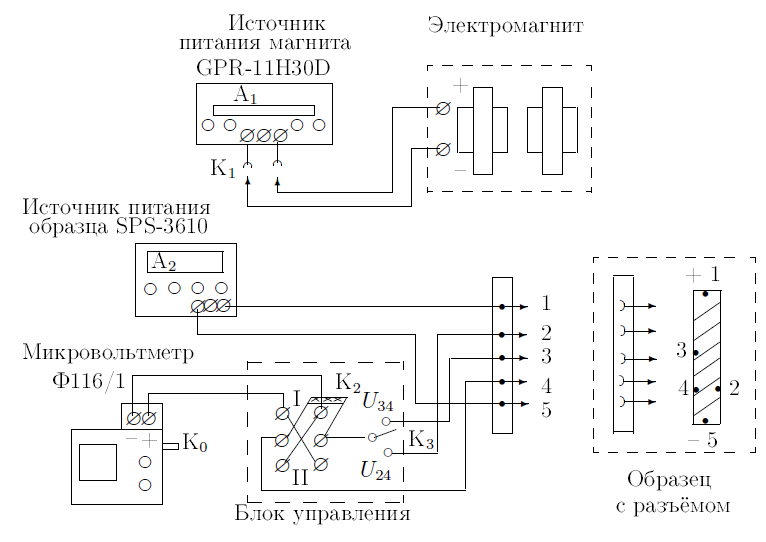
\includegraphics[width = \textwidth]{5.png}\\
\begin{center}
\textbf{Рисунок 1.}Схема установки для исследования эффекта Холла в металлах.
\end{center}
В зазоре электромагнита создается постоянное магнитное поле, которое можно регулировать с помощью источника питания электромагнита.\\
Иногда контакты 2 и 4 вследствие неточности подпайки не лежат на одной эквипотенциали, и тогда напряжение между ними связано не только с эффектом Холла, но и с омическим напряжением, вызванным протеканием основного тока через образец. \\
Неточности измерений можно избежать путем фиксирования этого омического напряжения при нулевом значении силы тока и отсчитывании от него Холловского напряжения. 
\[\varepsilon_x = U_{24} \pm U_0\]
Измерив ток в образце и нарпяжение $U_{34}$ между контактами 3 и 4 в отсутствии магнитного поля, можно, зная параметры образца, рассчитать проводимость материала образца по очевидной формуле:
\begin{equation}
\sigma = \dfrac{I L_{34}}{U_{34}al}
\end{equation}

\section{Ход работы}
\subsection{Калибровка}
Проводим измерение зависимости магнитного потока от величины силы тока. Результаты приведены в таблице и на графике ниже.\\
\begin{center}
\begin{tabular}{|c|c|c|c|c|}
\hline
 & $I_{\text{м}}, A$ & $\sigma_{I_{\text{м}}}, A$ & $B, \text{мТл}$ & $\sigma_{B}, \text{мТл}$ \\ \hline
1 & 0,19 & 0,01 & 252 & 5 \\ \hline
2 & 0,37 & 0,01 & 455 & 10 \\ \hline
3 & 0,56 & 0,01 & 678 & 10 \\ \hline
4 & 0,75 & 0,01 & 940 & 50 \\ \hline
5 & 0,94 & 0,01 & 1070 & 50 \\ \hline
6 & 1,13 & 0,01 & 1150 & 50 \\ \hline
\end{tabular}\\
\textbf{Таблица 1.}$B = f(I_{\text{м}})$

\end{center}
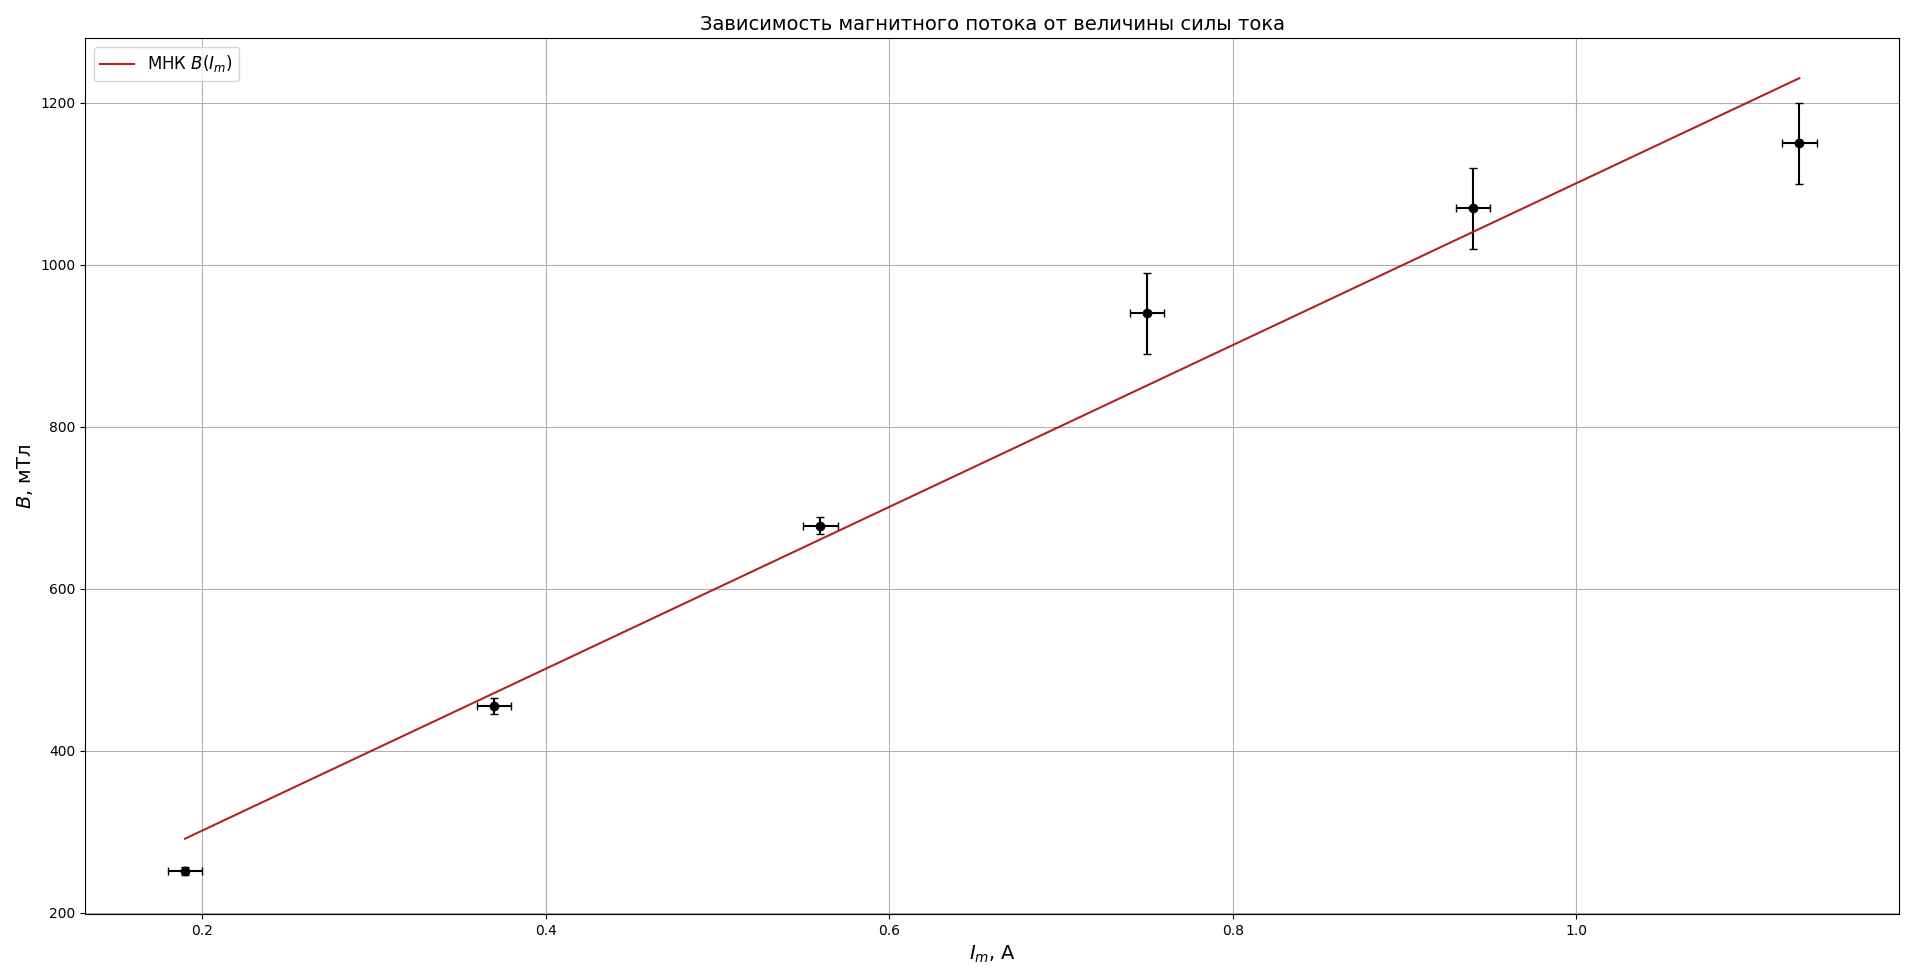
\includegraphics[width = \textwidth]{graph1.png}
\begin{center}
\textbf{График 1.}Нахождение $B = f(I_{\text{м}}$)
\end{center}

\subsection{Медь}

    \par Для начала отметим, что при измерении меди $75\; \text{дел} = 3\; \text{мкВ}$
    
    Проводим измерения ЭДС Холла. Для этого вставляем образец в зазор выключенного электромагнита и определяем $U_0$ между контактами 2 и 4. Это значение следует принять за 0.
    \par Далее включаем электромагнит и измеряем $U = f(I_{\text{м}})$ для образца из меди.

    Проводим серию для 8 значений тока через образец.\\
    То же делаем для образца из цинка при одном фиксированном значении тока через образец.\\
    Определяем знак носителей заряда для меди -- (\textbf{+}). \\
    $$L_{3,4} = 6\,\text{мм} \qquad a = 0.05\,\text{мм} \qquad l = 8\,\text{мм}$$ \\

    \begin{table}[H]
      \centering
      \caption{Для тока через материал $I = 0.20$ A}
      \label{tabular:med1}
        \begin{tabular}{|c|c|c|c|c|c|c|c|} \hline
            & \multicolumn{7}{c|}{$(I = 0.20 \pm 0.01)$ А, \qquad $U_0 = (11 \pm 1)$ ед.} \\ \hline
            & $I_{\text{м}}$, А & $\sigma_{I_{\text{м}}}, A$ & $B$, мТл & $\sigma_B$, мТл & $U$, ед. & $U$, нВ & $\sigma_{U}$, нВ \\ \hline
          1 & 0.19 & 0.01 &  190 & 11 & 11 & 440 & 20 \\ \hline
          2 & 0.37 & 0.01 &  370 & 13 & 12 & 480 & 20 \\ \hline
          3 & 0.56 & 0.01 &  559 & 14 & 14 & 560 & 20 \\ \hline
          4 & 0.75 & 0.01 &  749 & 15 & 15 & 600 & 20 \\ \hline
          5 & 0.94 & 0.01 &  939 & 17 & 16 & 640 & 20 \\ \hline
          6 & 1.13 & 0.01 & 1129 & 18 & 16 & 640 & 20 \\ \hline
          7 & 1.28 & 0.01 & 1279 & 19 & 16 & 640 & 20 \\ \hline
        \end{tabular}\\
    \end{table}

    \begin{table}[H]
      \centering
      \caption{Для тока через материал $I = 0.35$ A}
      \label{tabular:med2}
        \begin{tabular}{|c|c|c|c|c|c|c|c|} \hline
            & \multicolumn{7}{c|}{$(I = 0.35 \pm 0.01)$ А, \qquad $U_0 = (10 \pm 1)$ ед.} \\ \hline
            & $I_{\text{м}}$, А & $\sigma_{I_{\text{м}}}, A$ & $B$, мТл & $\sigma_B$, мТл & $U$, ед. & $U$, нВ & $\sigma_{U}$, нВ \\ \hline
          1 & 0.19 & 0.01 &  190 & 11 & 12 & 480 & 20 \\ \hline
          2 & 0.37 & 0.01 &  370 & 13 & 14 & 560 & 20 \\ \hline
          3 & 0.56 & 0.01 &  559 & 14 & 16 & 640 & 20 \\ \hline
          4 & 0.75 & 0.01 &  749 & 15 & 18 & 720 & 20 \\ \hline
          5 & 0.94 & 0.01 &  939 & 17 & 19 & 760 & 20 \\ \hline
          6 & 1.13 & 0.01 & 1129 & 18 & 20 & 800 & 20 \\ \hline
          7 & 1.26 & 0.01 & 1259 & 19 & 21 & 840 & 20 \\ \hline
        \end{tabular}\\
    \end{table}

    \begin{table}[H]
      \centering
      \caption{Для тока через материал $I = 0.50$ A}
      \label{tabular:med3}
        \begin{tabular}{|c|c|c|c|c|c|c|c|} \hline
            & \multicolumn{7}{c|}{$(I = 0.50 \pm 0.01)$ А, \qquad $U_0 = (10 \pm 1)$ ед.} \\ \hline
            & $I_{\text{м}}$, А & $\sigma_{I_{\text{м}}}, A$ & $B$, мТл & $\sigma_B$, мТл & $U$, ед. & $U$, нВ & $\sigma_{U}$, нВ \\ \hline
          1 & 0.19 & 0.01 &  190 & 11 & 14.5 & 580 & 20 \\ \hline
          2 & 0.37 & 0.01 &  370 & 13 & 18 & 720 & 20 \\ \hline
          3 & 0.56 & 0.01 &  559 & 14 & 21 & 840 & 20 \\ \hline
          4 & 0.75 & 0.01 &  749 & 15 & 24 & 960 & 20 \\ \hline
          5 & 0.94 & 0.01 &  939 & 17 & 26 & 1040 & 20 \\ \hline
          6 & 1.13 & 0.01 & 1129 & 18 & 27 & 1080 & 20 \\ \hline
          7 & 1.26 & 0.01 & 1259 & 19 & 28 & 1120 & 20 \\ \hline
        \end{tabular}\\
    \end{table}

    \begin{table}[H]
      \centering
      \caption{Для тока через материал $I = 0.65$ A}
      \label{tabular:med4}
        \begin{tabular}{|c|c|c|c|c|c|c|c|} \hline
            & \multicolumn{7}{c|}{$(I = 0.65 \pm 0.01)$ А, \qquad $U_0 = (11 \pm 1)$ ед.} \\ \hline
            & $I_{\text{м}}$, А & $\sigma_{I_{\text{м}}}, A$ & $B$, мТл & $\sigma_B$, мТл & $U$, ед. & $U$, нВ & $\sigma_{U}$, нВ \\ \hline
          1 & 0.19 & 0.01 &  190 & 11 & 15.5 & 620 & 20 \\ \hline
          2 & 0.37 & 0.01 &  370 & 13 & 19 & 760 & 20 \\ \hline
          3 & 0.56 & 0.01 &  559 & 14 & 24 & 960 & 20 \\ \hline
          4 & 0.75 & 0.01 &  749 & 15 & 28 & 1120 & 20 \\ \hline
          5 & 0.94 & 0.01 &  939 & 17 & 30 & 1200 & 20 \\ \hline
          6 & 1.13 & 0.01 & 1129 & 18 & 32 & 1280 & 20 \\ \hline
          7 & 1.26 & 0.01 & 1259 & 19 & 33 & 1320 & 20 \\ \hline
        \end{tabular}\\
    \end{table}

    \begin{table}[H]
      \centering
      \caption{Для тока через материал $I = 0.80$ A}
      \label{tabular:med5}
        \begin{tabular}{|c|c|c|c|c|c|c|c|} \hline
            & \multicolumn{7}{c|}{$(I = 0.80 \pm 0.01)$ А, \qquad $U_0 = (12 \pm 1)$ ед.} \\ \hline
            & $I_{\text{м}}$, А & $\sigma_{I_{\text{м}}}, A$ & $B$, мТл & $\sigma_B$, мТл & $U$, ед. & $U$, нВ & $\sigma_{U}$, нВ \\ \hline
          1 & 0.19 & 0.01 &  190 & 11 & 17 & 680 & 20 \\ \hline
          2 & 0.37 & 0.01 &  370 & 13 & 23 & 920 & 20 \\ \hline
          3 & 0.56 & 0.01 &  559 & 14 & 28 & 1120 & 20 \\ \hline
          4 & 0.75 & 0.01 &  749 & 15 & 32 & 1280 & 20 \\ \hline
          5 & 0.94 & 0.01 &  939 & 17 & 36 & 1440 & 20 \\ \hline
          6 & 1.16 & 0.01 & 1159 & 18 & 38 & 1520 & 20 \\ \hline
          7 & 1.26 & 0.01 & 1259 & 19 & 39 & 1560 & 20 \\ \hline
        \end{tabular}\\
    \end{table}

    \begin{table}[H]
      \centering
      \caption{Для тока через материал $I = 0.95$ A}
      \label{tabular:med6}
        \begin{tabular}{|c|c|c|c|c|c|c|c|} \hline
            & \multicolumn{7}{c|}{$(I = 0.95 \pm 0.01)$ А, \qquad $U_0 = (13 \pm 1)$ ед.} \\ \hline
            & $I_{\text{м}}$, А & $\sigma_{I_{\text{м}}}, A$ & $B$, мТл & $\sigma_B$, мТл & $U$, ед. & $U$, нВ & $\sigma_{U}$, нВ \\ \hline
          1 & 0.19 & 0.01 &  190 & 11 & 19 & 760 & 20 \\ \hline
          2 & 0.37 & 0.01 &  370 & 13 & 25 & 1000 & 20 \\ \hline
          3 & 0.56 & 0.01 &  559 & 14 & 32 & 1280 & 20 \\ \hline
          4 & 0.74 & 0.01 &  739 & 15 & 38 & 1520 & 20 \\ \hline
          5 & 0.94 & 0.01 &  939 & 17 & 42 & 1680 & 20 \\ \hline
          6 & 1.16 & 0.01 & 1159 & 18 & 45 & 1800 & 20 \\ \hline
          7 & 1.25 & 0.01 & 1249 & 19 & 46 & 1840 & 20 \\ \hline
        \end{tabular}\\
    \end{table}

    \begin{table}[H]
      \centering
      \caption{Для тока через материал $I = 1.10$ A}
      \label{tabular:med7}
        \begin{tabular}{|c|c|c|c|c|c|c|c|} \hline
            & \multicolumn{7}{c|}{$(I = 1.10 \pm 0.01)$ А, \qquad $U_0 = (14 \pm 1)$ ед.} \\ \hline
            & $I_{\text{м}}$, А & $\sigma_{I_{\text{м}}}, A$ & $B$, мТл & $\sigma_B$, мТл & $U$, ед. & $U$, нВ & $\sigma_{U}$, нВ \\ \hline
          1 & 0.19 & 0.01 &  190 & 11 & 21 & 840 & 20 \\ \hline
          2 & 0.37 & 0.01 &  370 & 13 & 28 & 1120 & 20 \\ \hline
          3 & 0.56 & 0.01 &  559 & 14 & 36 & 1440 & 20 \\ \hline
          4 & 0.74 & 0.01 &  739 & 15 & 43 & 1720 & 20 \\ \hline
          5 & 0.94 & 0.01 &  939 & 17 & 47 & 1880 & 20 \\ \hline
          6 & 1.16 & 0.01 & 1159 & 18 & 50 & 2000 & 20 \\ \hline
          7 & 1.25 & 0.01 & 1249 & 19 & 51 & 2040 & 20 \\ \hline
        \end{tabular}\\
    \end{table}

    \begin{table}[H]
      \centering
      \caption{Для тока через материал $I = 1.25$ A}
      \label{tabular:med8}
        \begin{tabular}{|c|c|c|c|c|c|c|c|} \hline
            & \multicolumn{7}{c|}{$(I = 1.25 \pm 0.01)$ А, \qquad $U_0 = (-6 \pm 1)$ ед.} \\ \hline
            & $I_{\text{м}}$, А & $\sigma_{I_{\text{м}}}, A$ & $B$, мТл & $\sigma_B$, мТл & $U$, ед. & $U$, нВ & $\sigma_{U}$, нВ \\ \hline
          1 & 0.19 & 0.01 &  190 & 11 & 23 & 920 & 20 \\ \hline
          2 & 0.37 & 0.01 &  370 & 13 & 32 & 1280 & 20 \\ \hline
          3 & 0.56 & 0.01 &  559 & 14 & 41 & 1640 & 20 \\ \hline
          4 & 0.75 & 0.01 &  749 & 15 & 49 & 1960 & 20 \\ \hline
          5 & 0.93 & 0.01 &  929 & 17 & 53 & 2120 & 20 \\ \hline
          6 & 1.14 & 0.01 & 1139 & 18 & 57 & 2280 & 20 \\ \hline
          7 & 1.24 & 0.01 & 1239 & 19 & 58 & 2320 & 20 \\ \hline
        \end{tabular}\\
    \end{table}

    \begin{figure}[h]
      \centering
        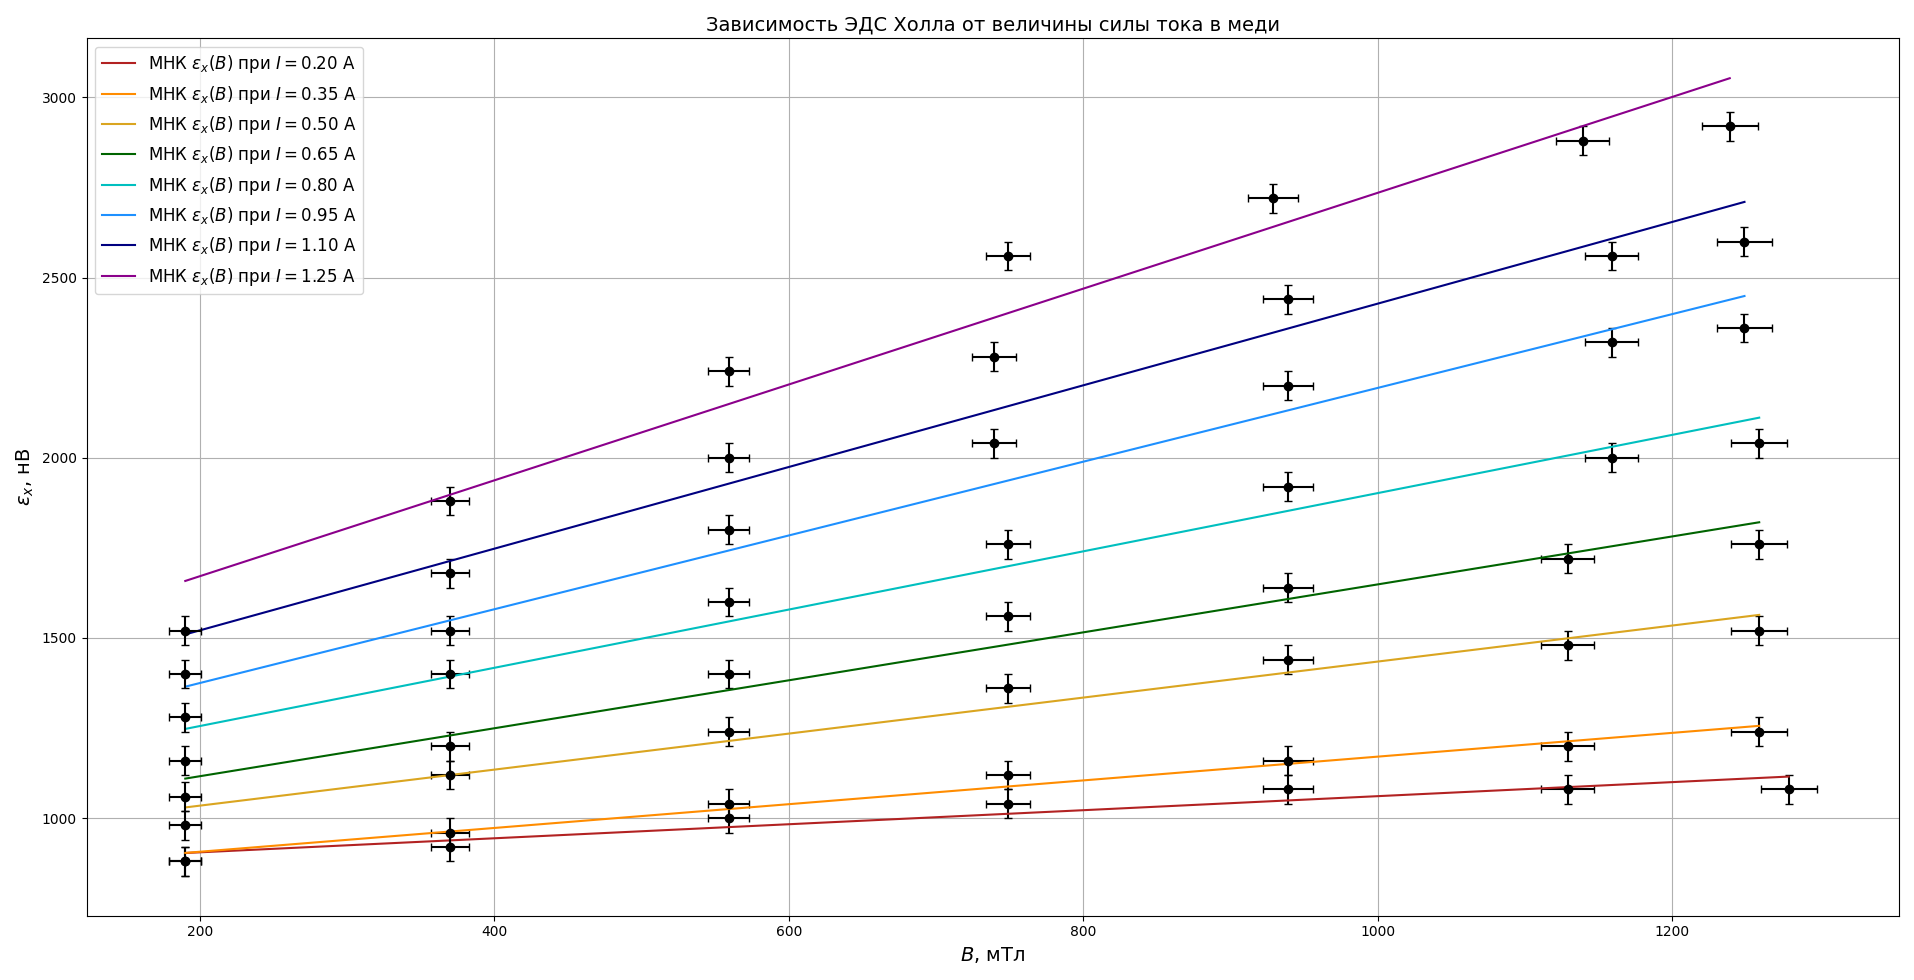
\includegraphics[scale=0.38]{graph-hall-med.png}
      \caption{График $\varepsilon_x = f(B)$ для меди}
    \end{figure}

    Далее находим функцию зависимости $k = f(I)$, где $k$ - коэффициент угла наклона для каждого из токов.\\

    \begin{table}[H]
      \centering
      \caption{Функция $k = f(I)$}
      \label{tabular:med}
        \begin{tabular}{|c|c|c|c|c|} \hline
          & $I$, A & $\sigma_{I}$, A & $k$, $\dfrac{\text{мкВ}}{\text{Тл}}$ & $\sigma_k$, $\dfrac{\text{мкВ}}{\text{Тл}}$ \\ \hline
        1 & 0.20 & 0.01 & 0.195 & 0.005 \\ \hline
        2 & 0.35 & 0.01 & 0.330 & 0.005 \\ \hline
        3 & 0.50 & 0.01 & 0.500 & 0.005 \\ \hline
        4 & 0.65 & 0.01 & 0.665 & 0.005 \\ \hline
        5 & 0.80 & 0.01 & 0.808 & 0.005 \\ \hline
        6 & 0.95 & 0.01 & 1.024 & 0.005 \\ \hline
        7 & 1.10 & 0.01 & 1.133 & 0.005 \\ \hline
        8 & 1.25 & 0.01 & 1.330 & 0.005 \\ \hline
        \end{tabular}\\
    \end{table}

    \begin{figure}[h]
      \centering
        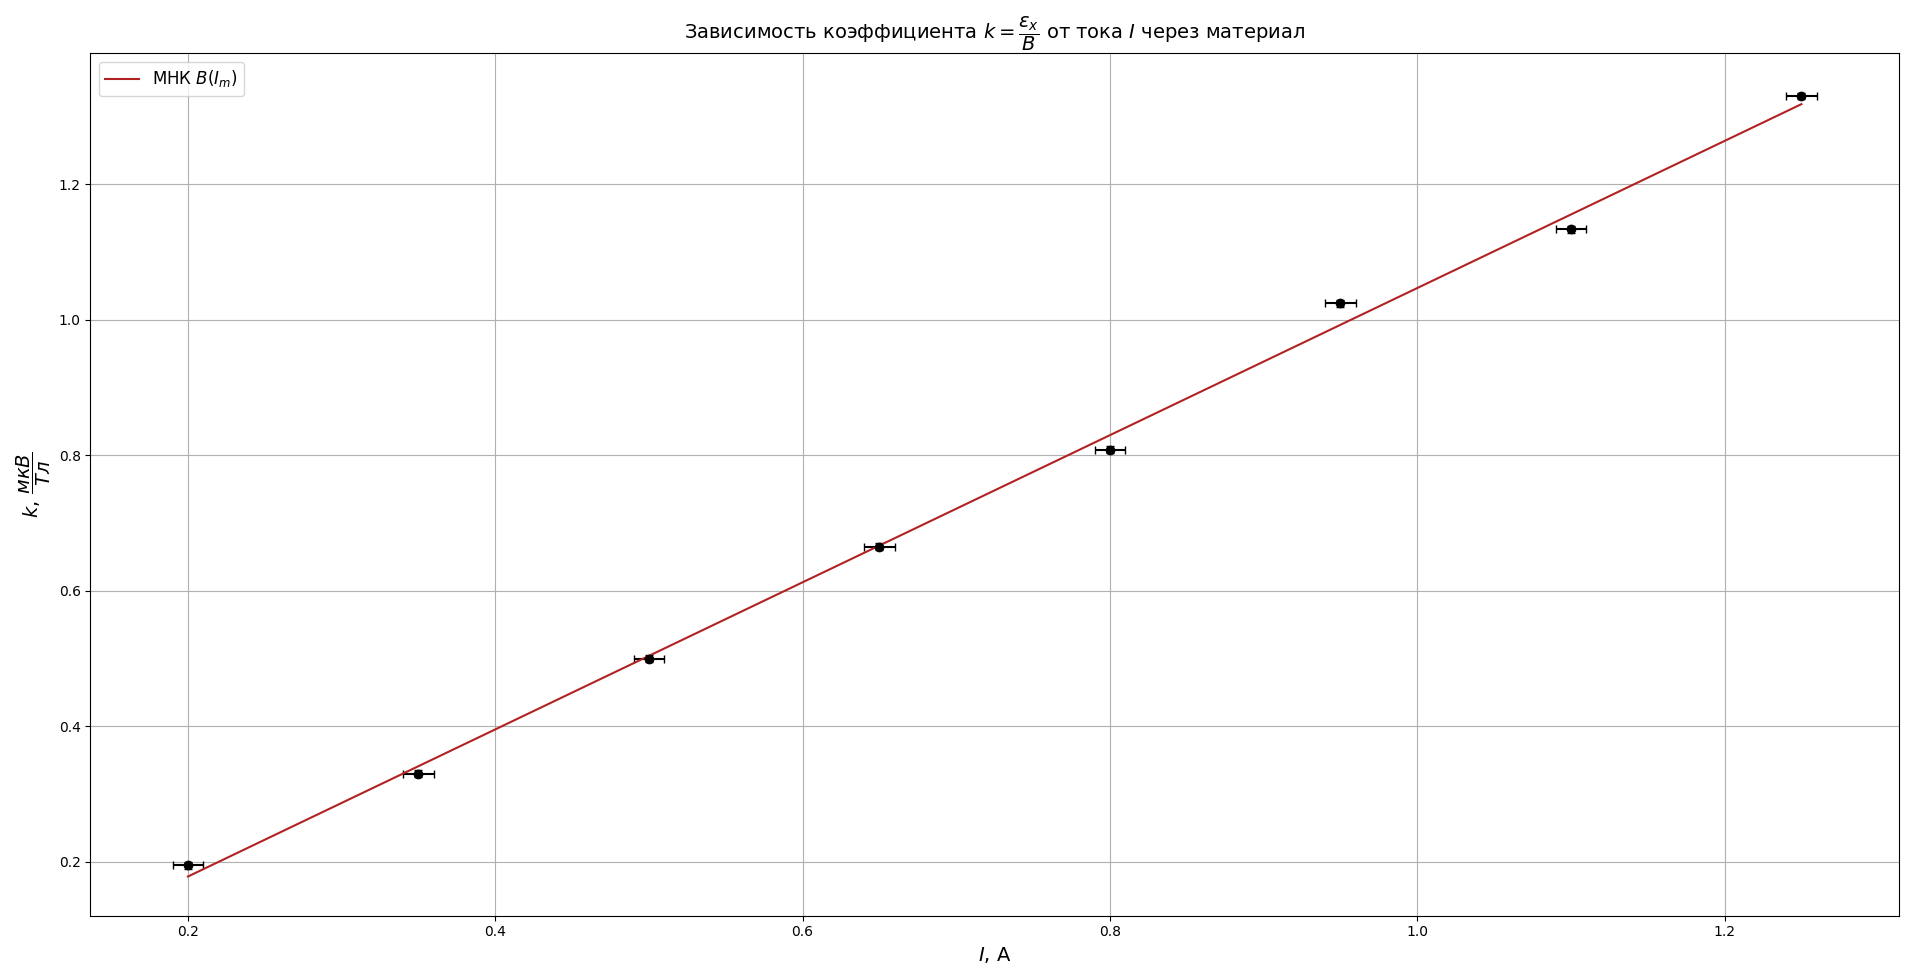
\includegraphics[scale=0.38]{graph-ki.png}
      \caption{График $k = f(I)$}
    \end{figure}

    Из угла наклона графика зависимости $k = f(I)$ мы получаем, что угол наклона этого графика $K^{Cu} = (1.08 \pm 0.02) \dfrac{\text{мкОм}}{\text{Тл}}$\\
    Из этого мы получаем, что из формулы во введении следует, что 
    $$R_x^{Cu} = -K^{Cu} \cdot a = -(5.4 \pm 0.1) \cdot 10^{-11} \dfrac{\text{м}^3}{\text{Кл}}$$
    Как видим, полученное нами значение хорошо совпадает с табличным $ R_x^{Cu,\,th} = -5.5 \cdot 10^{-11} \dfrac{\text{м}^3}{\text{Кл}}$

    \subsection{Цинк}
    Для начала отметим, что при измерении цинка $75\text{дел} = 7.5\text{мкВ}$.
    Определяем знак носителей заряда для цинка -- (\textbf{-}). \\
    $$L_{3,4} = 3.5\,\text{мм} \qquad a = 0.12\,\text{мм} \qquad l = 9\,\text{мм}$$ \\

    \begin{table}[H]
      \centering
      \caption{Для тока через материал $I = 1.00$ A}
      \label{tabular:zink1}
        \begin{tabular}{|c|c|c|c|c|c|c|c|} \hline
            & \multicolumn{7}{c|}{$(I = 1.00 \pm 0.01)$ А, \qquad $U_0 = (13 \pm 1)$ ед.} \\ \hline
            & $I_{\text{м}}$, А & $\sigma_{I_{\text{м}}}, A$ & $B$, мТл & $\sigma_B$, мТл & $U$, ед. & $U$, нВ & $\sigma_{U}$, нВ \\ \hline
          1 & 0.19 & 0.01 &  190 & 11 & 16 & 1600 & 50 \\ \hline
          2 & 0.37 & 0.01 &  370 & 13 & 19 & 1900 & 50 \\ \hline
          3 & 0.56 & 0.01 &  559 & 14 & 22 & 2200 & 50 \\ \hline
          4 & 0.74 & 0.01 &  739 & 15 & 24 & 2400 & 50 \\ \hline
          5 & 0.93 & 0.01 &  929 & 17 & 26 & 2600 & 50 \\ \hline
          6 & 1.16 & 0.01 & 1159 & 18 & 27 & 2700 & 50 \\ \hline
          7 & 1.25 & 0.01 & 1249 & 19 & 28 & 2800 & 50 \\ \hline
        \end{tabular}\\
    \end{table}

    \begin{figure}[h]
      \centering
        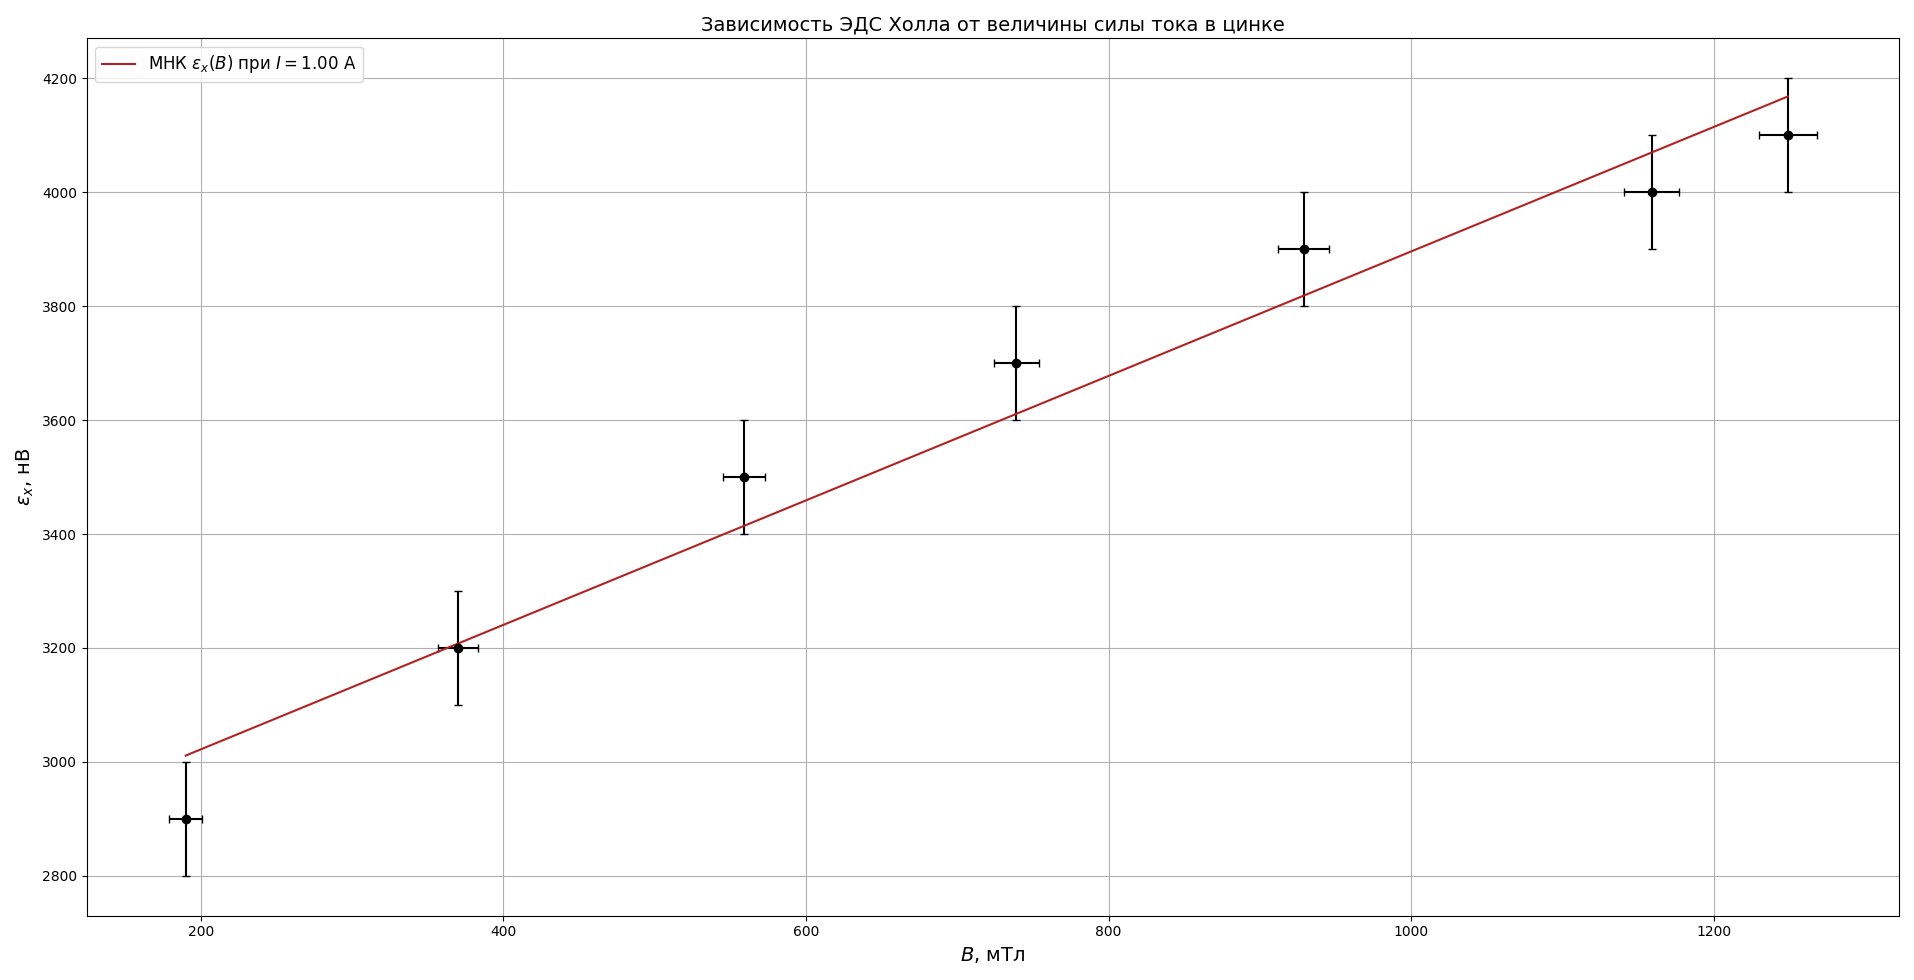
\includegraphics[scale=0.38]{graph-hall-zink.png}
      \caption{График $\varepsilon_x = f(B)$ для цинка}
    \end{figure}

    Теперь ищем то же самое для цинка: 
    $$K^{Zn} = (1.1 \pm 0.3) \dfrac{\text{мкВ}}{\text{Тл}}$$
    $$R_x^{Zn} = - \dfrac{K^{Zn} \cdot a}{I} = (1.3 \pm 0.4) \cdot 10^{-10} \dfrac{\text{м}^3}{\text{Кл}}$$
    Сравнивая с табличным значением, видим, что наше значение, с учетом погрешности, совпадает с табличным $R_x^{Zn,\,th} = +1,04 \cdot 10^{-10} \dfrac{\text{м}^3}{\text{Кл}}$\\


    \subsection{Серебро}
    Для начала отметим, что при измерении серебра $75\text{дел} = 1.5\text{мкВ}$.
    Определяем знак носителей заряда для серебра -- (\textbf{+}) . \\
    $$L_{3,4} = 15\,\text{мм} \qquad a = 0.09\,\text{мм} \qquad l = 11\,\text{мм}$$ \\

    \begin{table}[H]
      \centering
      \caption{Для тока через материал $I = 1.00$ A}
      \label{tabular:arg1}
        \begin{tabular}{|c|c|c|c|c|c|c|c|} \hline
            & \multicolumn{7}{c|}{$(I = 1.00 \pm 0.01)$ А, \qquad $U_0 = (-3 \pm 1)$ ед.} \\ \hline
            & $I_{\text{м}}$, А & $\sigma_{I_{\text{м}}}, A$ & $B$, мТл & $\sigma_B$, мТл & $U$, ед. & $U$, нВ & $\sigma_{U}$, нВ \\ \hline
          1 & 0.19 & 0.01 &  190 & 11 & 7 & 140 & 10 \\ \hline
          2 & 0.37 & 0.01 &  370 & 13 & 19 & 380 & 10 \\ \hline
          3 & 0.56 & 0.01 &  559 & 14 & 30 & 600 & 10 \\ \hline
          4 & 0.74 & 0.01 &  739 & 15 & 40 & 800 & 10 \\ \hline
          5 & 0.93 & 0.01 &  929 & 17 & 47 & 940 & 10 \\ \hline
          6 & 1.16 & 0.01 & 1159 & 18 & 51 & 1020 & 10 \\ \hline
          7 & 1.25 & 0.01 & 1249 & 19 & 52 & 1040 & 10 \\ \hline
        \end{tabular}\\
    \end{table}

    \begin{figure}[h]
      \centering
        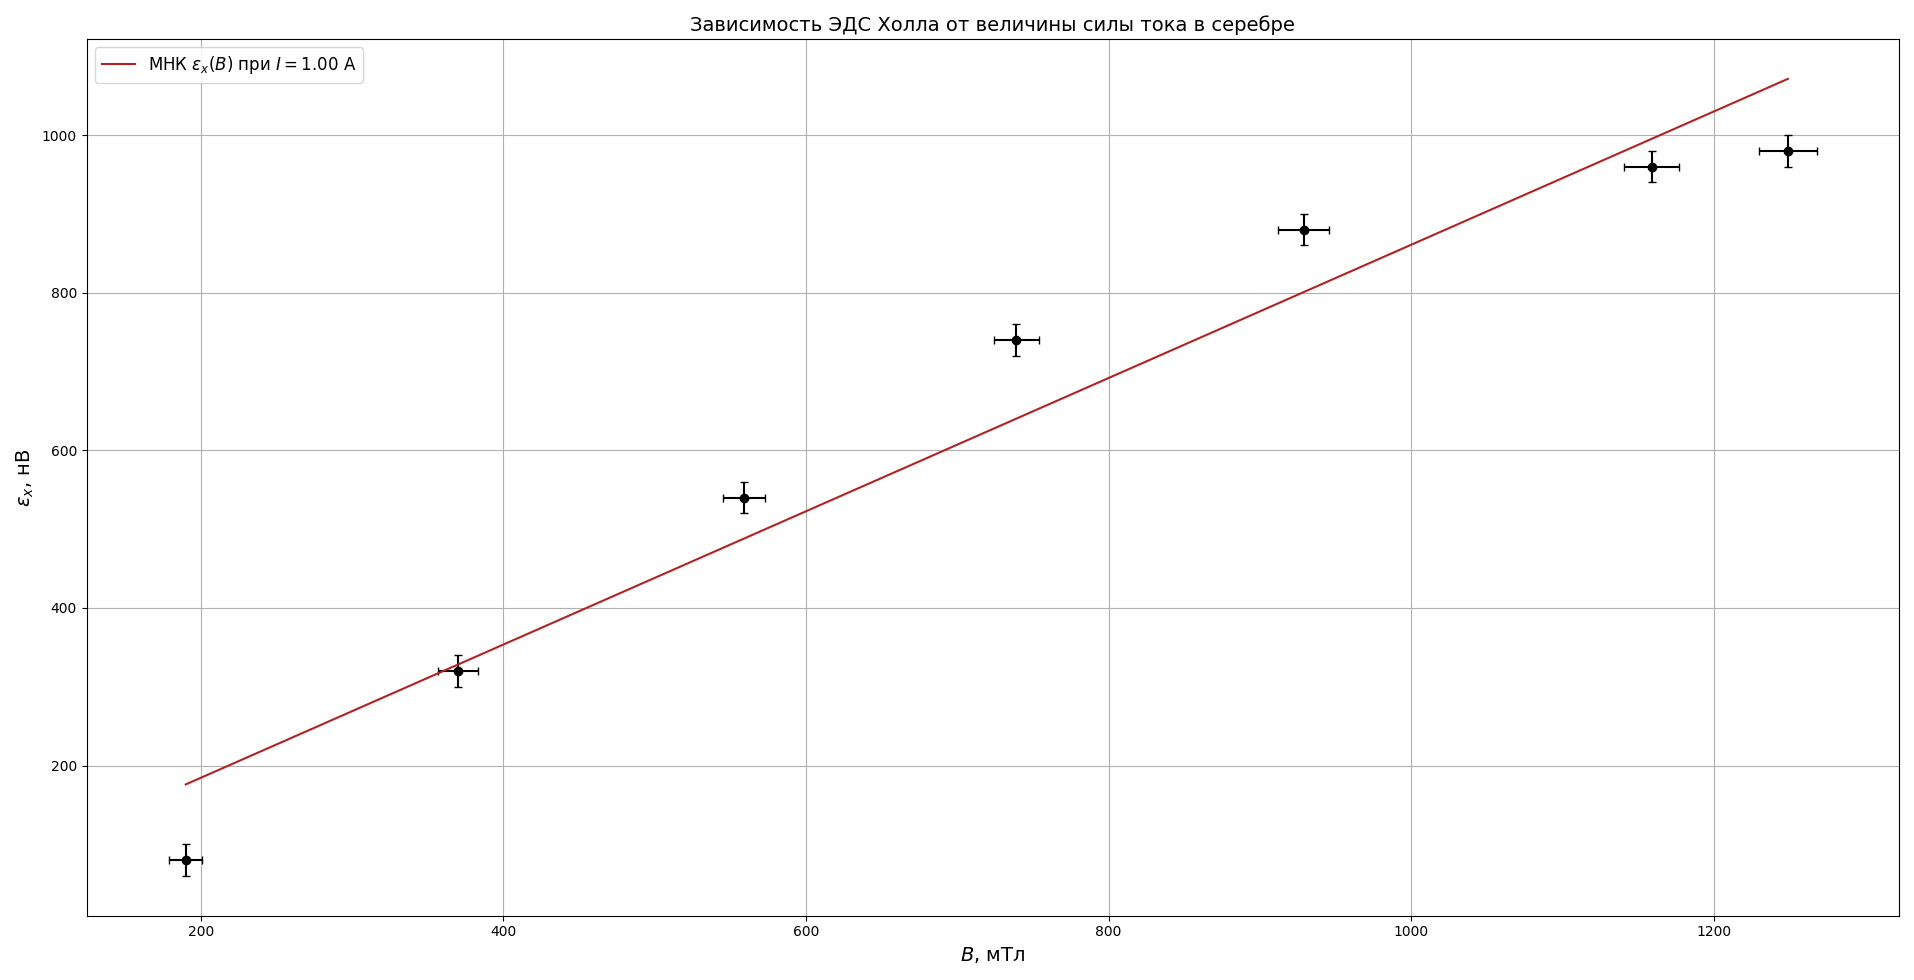
\includegraphics[scale=0.38]{graph-hall-arg.png}
      \caption{График $\varepsilon_x = f(B)$ для серебра}
    \end{figure}

    Теперь ищем то же самое для серебра: 
    $$K^{Ag}  = (0.85 \pm 0.15) \dfrac{\text{мкВ}}{\text{Тл}}$$
    $$R_x^{Ag} = - \dfrac{K^{Ag} \cdot a}{I} = (-7.7 \pm 1.4) \cdot 10^{-11} \dfrac{\text{м}^3}{\text{Кл}}$$
    Сравнивая с табличным значением, видим, что наше значение, с учетом погрешности, совпадает с табличным $R_x^{Ag,\,th} = -0.9 \cdot 10^{-10} \dfrac{\text{м}^3}{\text{Кл}}$\\


    \subsection{Концентрация носителей тока и удельная проводимость}
    
    Далее рассчитаем концентрацию носителей тока по формуле (6)\\
    
    Рассчитаем удельную проводимость $\sigma$ для образцов по формуле (7).\\
   
    Используя найденные значения рассчитываем подвижность носителей по формуле 
    \[b = \dfrac{\sigma}{n \cdot e} = R_x \cdot \sigma\]

    Занесём данные в таблицу 

    \begin{table}[h!]
        \begin{tabular}{|l|l|l|l|l|l|l|}
            \hline
            Металл  & R $\pm \Delta R, 10^{-11} \frac{\text{м}^3}{\text{Кл}}$       & Табл. R,  $ 10^{-11} \frac{\text{м}^3}{\text{Кл}}$ & Знак & n$\pm \Delta n, 10^{30}\frac{1}{\text{м}^3}$         & $\sigma \pm \Delta \sigma, 10^{8}\frac{1}{\text{Ом$\cdot$м}}$    & b, $\frac{\text{см}^2}{\text{Ом$\cdot$м}}$   \\ \hline
            Медь    & -5,4$\pm$0,1 & -5,5     & +           & -0,12$\pm$0,01 & 0,48$\pm$0,06 & 26$\pm$3 \\ \hline
            Цинк    & 13 $\pm$4  & 10,4      & --           & 0,05$\pm$0,01 & 0,07$\pm$0,01 & 9,1$\pm$2,8 \\ \hline
            Серебро & -7,7$\pm$1,4 & -9.0       & +           &  -0,08$\pm$0,01         &    0,40$\pm$0,05       &  31  $\pm$ 6  \\ \hline
        \end{tabular}
    \end{table}

    
    \section{Вывод}
    Найденнае нами постоянные Холла с учётом погрешности совпадают с табличными. Знак этой постоянной показывает, что основными носителями заряда в меди и серебре являются электроны, а в цинке дырки.

\end{document}
